%%% Работа с русским языком
\usepackage{cmap}					% поиск в PDF
\usepackage[T2A]{fontenc}			% кодировка
\usepackage[utf8]{inputenc}			% кодировка исходного текста
\usepackage[english,russian]{babel}	% локализация и переносы
\usepackage{indentfirst}
\frenchspacing

\usepackage{subfigure}

%%% Дополнительная работа с математикой
\usepackage{amsmath,amsfonts,amssymb,amsthm,mathtools} % AMS
\usepackage{icomma} % "Умная" запятая: $0,2$ --- число, $0, 2$ --- перечисление

%%% Работа с картинками
\usepackage{graphicx}  % Для вставки рисунков
\usepackage{wrapfig} % Обтекание рисунков текстом
\usepackage{subfigure}

%%% Работа с таблицами
\usepackage{array,tabularx,tabulary,booktabs} % Дополнительная работа с таблицами
\usepackage{longtable}  % Длинные таблицы
\usepackage{multirow} % Слияние строк в таблице

%%% Программирование
\usepackage{etoolbox} % логические операторы


\usepackage{setspace} % Интерлиньяж
%\onehalfspacing % Интерлиньяж 1.5
%\doublespacing % Интерлиньяж 2
%\singlespacing % Интерлиньяж 1

\usepackage{lastpage} % Узнать, сколько всего страниц в документе.

\usepackage{soul} % Модификаторы начертания

\usepackage{tikz} % Работа с графикой
\usepackage{pgfplots}
\usepackage{pgfplotstable}

\renewcommand{\phi}{\varphi}
\renewcommand{\epsilon}{\varepsilon}
\usepackage[backend=biber, sorting=none]{biblatex}
\usepackage{subfigure}

\addbibresource{lit.bib}

\theoremstyle{definition}
\newtheorem*{Def}{Определение}
\theoremstyle{plain}
\newtheorem{Lem}{Лемма}
\newtheorem{Th}{Теорема}

\usepackage{listings}

\definecolor{codegreen}{rgb}{0,0.6,0}
\definecolor{codegray}{rgb}{0.5,0.5,0.5}
\definecolor{codepurple}{rgb}{0.58,0,0.82}
\definecolor{backcolour}{rgb}{0.95,0.95,0.92}

\lstdefinestyle{mystyle}{
	backgroundcolor=\color{backcolour},   
	commentstyle=\color{codegreen},
	keywordstyle=\color{magenta},
	numberstyle=\tiny\color{codegray},
	stringstyle=\color{codepurple},
	basicstyle=\ttfamily\footnotesize,
	breakatwhitespace=false,         
	breaklines=true,                 
	captionpos=b,                    
	keepspaces=true,                 
	numbers=left,                    
	numbersep=5pt,                  
	showspaces=false,                
	showstringspaces=false,
	showtabs=false,                  
	tabsize=2
}

\lstset{style=mystyle}

\newcommand{\delayV}[1]{\overset{\leftarrow}{\mathbf{x}}_{#1}}
\newcommand{\delayM}[1]{\overset{\leftarrow}{\mathbf{X}}_{#1}}

\title{Тензорная декомпозиция и прогноз для набора временных рядов}
\author{Сёмкин Кирилл$^{1}$ \\ {\footnotesize $^{1}$semkin.ki@phystech.edu} \and Вадим Стрижов$^{2}$ \\ {\footnotesize $^{2}$vadim.swifton@gmail.com}}
\date{}


\begin{document}
	
	\maketitle
	
	\begin{abstract}
		
		Декомпозиция временного ряда применяется для получения его структуры: разложения на простые и/или интерпретируемые составляющие, выявление периодичности, избавление от шума и т.д. В случае же набора нескольких рядов игнорирование взаимосвязей между ними может приводить к некачественным, ложным разложениям и предсказаниям. В данной работе предлагается метод декомпозиции, учитывающий фактор связанности и основанный на классическом методе SSA (Гусеница) и тензорных разложениях, а также способ прогноза будущих значений ряда. Предложенный подход сравнивается с методом mSSA, основанным на матричных разложениях, и рекуррентными нейросетями. Производится сравнение методов при обработке реальных данных (потребление электроэнергии, акселерометрия).
		
	\end{abstract}
	
	\textbf{Ключевые слова}: {\small временные ряды, декомпозиция, прогноз, SVD, SSA, каноническое тензорное разложение}.
	
	
	\section{Введение}\label{Intro}
	
		Настоящая работа посвящена методам декомпозиции и построения прогноза для \textit{набора временных рядов} --- нескольких рассматриваемых вместе сигналов $ \{x_i(t)\}_{i=1}^m $, где $ t \in 1 \ldots N $. Нас будет интересовать аддитивная декомпозиция --- представление ряда в виде суммы нескольких составляющих.
		
		Методы разложения~\cite{enders2010applied, x11, cleveland90} и прогнозирования~\cite{3b1355aedd1041f1853e609a410576f3, enders2010applied, Box_Jenkins_methodology} для одиночного сигнала не могут быть просто перенесены на наборы временных рядов в случае их взаимной зависимости друг от друга. Для иллюстрации достаточно взять модель хищник-жертва \cite{Volterra:1928}. Размер популяции одних особей зависит от размера популяции других и наоборот. Мы будем предполагать некую связь рядов, строгое определение которой будет даваться в рамках рассматриваемых далее моделей. Выявление же этой связи --- отдельная задача, см., например,~\cite{702ab909-8cb1-3c30-a5f1-ab4517d6cf1c, 2012Sci...338..496S}.
		
		Рассмотрим несколько подходов к поставленному вопросу. Модель \textit{рекуррентных нейронных сетей} (RNN) \cite{neco, TEALAB2018334} связывает ряды друг с другом и своими предыдущими реализациями композицией множества однотипных нелинейных преобразований. На каждом шаге происходит вычисление скрытого представления, инкапсулирующего в себе всю информацию о прошлом. С его помощью строится предсказания будущих значений рядов \cite{ZHANG2023143, HEWAMALAGE2021388}. 
		
		\textit{Векторная авторегрессия} (VAR)~\cite{VAR_model1, doi:10.1080/01621459.1962.10480664} представляет собой линейную стохастическую модель динамики набора временных рядов. Если из значений сигналов в момент $ t $ составить вектор $ \mathbf{x}_t = (x_1(t) \ldots x_m(t))^{\mathsf{T}} $, то динамика имеет вид:
		
		\begin{equation*}
			\mathbf{x}_t = \boldsymbol{\mu} + \sum\limits_{i = 1}^p A_i \mathbf{x}_{t - i} + \mathbf{u}_t
		\end{equation*}
		
		Здесь $ \boldsymbol{\mu} $ - некоторый константный вектор, $ A_i $ матрицы $ m \times m $, $ \mathbf{u}_t $ - случайный вектор (например, реализация белого шума $ \text{WN}(t) $). Как мы видим, связь рядов задаётся линейными преобразованиями $ A_i $, и каждый сигнал зависит как от собственных значений в прошлом, так и от прошлого других сигналов \textit{линейным образом}. 	
		
		Рассмотренные решения позволяют строить прогноз, но имеют большое количество подбираемых гиперпараметров и требуют затратных процедур обучения. Более того, структура этих моделей не содержит способа построения декомпозиции временных рядов. 
		
		В связи с этим мы разработали новый метод \emph{tSSA}, имеющий всего одну настраиваемую переменную и основывающийся на каноническом тензорном разложении CPD~\cite{kolda_tensors}. Его вычисление --- единственная необходимая процедура для получения декомпозиции и предсказания. Наш подход является расширением метода SSA~\cite{ecfb9dc578be43ae9ee8fc88b8ff9151} для многомерных временных рядов и опирается на теорию динамических систем: за основу взята модель \textit{собственного пространства сигнала}~\cite{1572261550523548160}. Она опирается на построение фазового представления временных рядов, иллюстрация на рис.\ref{pic:phase_traj}. Существует также другая модификация --- mSSA~\cite{mSSA_overview}, которое мы сравним с нашей в плане построения базиса в пространстве сигналов.
		
		\begin{figure}[h]
			\centering
			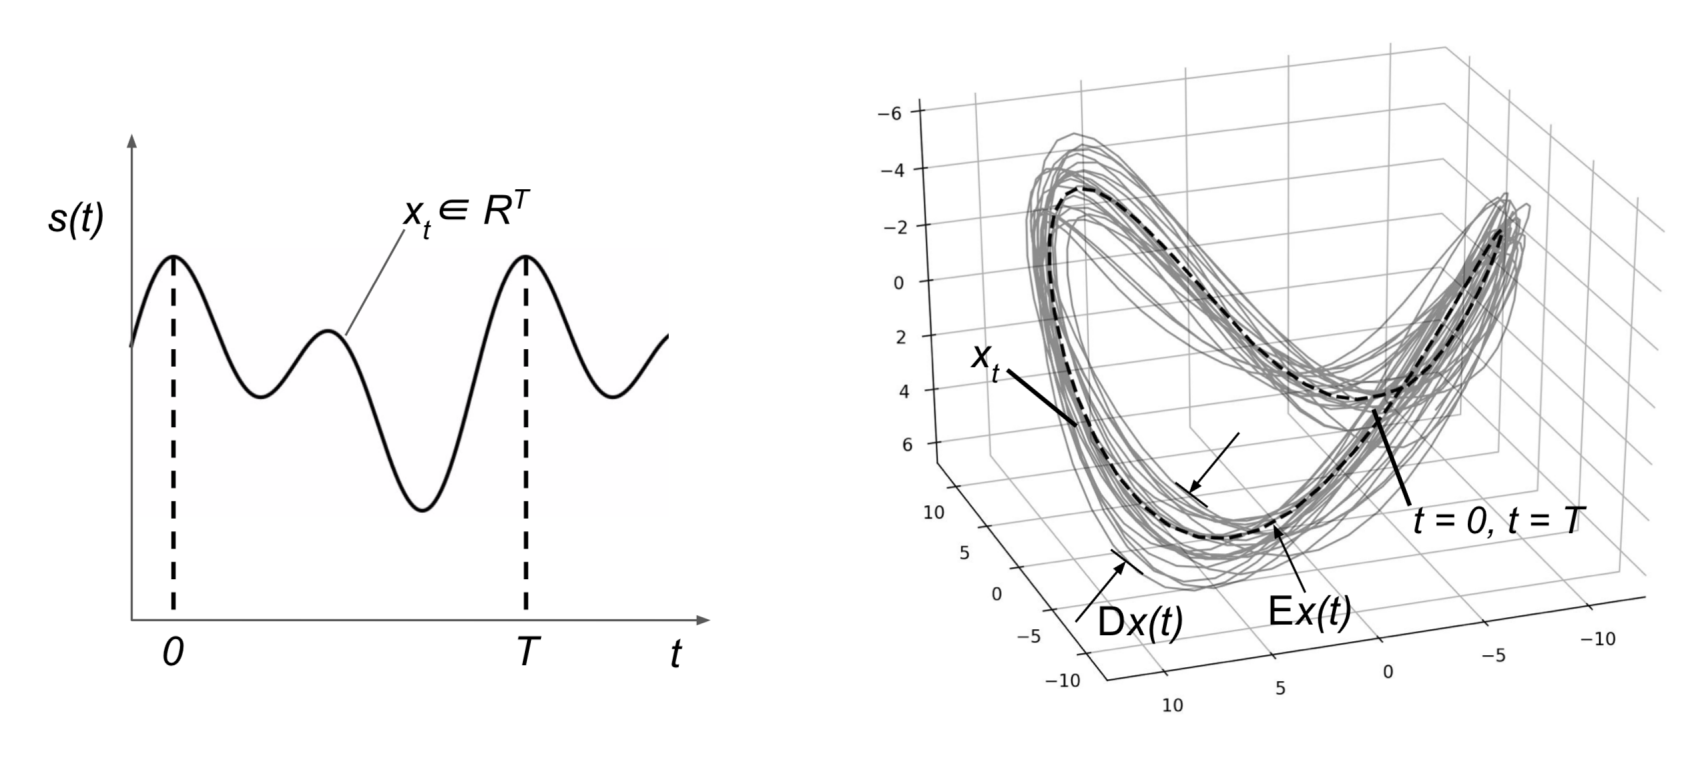
\includegraphics[width=0.9\textwidth, keepaspectratio]{../figs/phase_traj.png}
			\caption{Пример построения фазовой траектории временного ряда}\label{pic:phase_traj}
		\end{figure}
		
		Далее в работе будет формально введена математическая модель порождения временных рядов, поставлена задача поиска базиса в пространстве сигналов и предложено её решение. На его основе будет рассмотрен наш способ построения декомпозиции и прогноза для рядов, а также проанализированы его свойства и вычислительные особенности. Далее рассмотренные выше методы будут применены к реальным данным потребления электроэнергии и $ TODO $, будут проанализированы их точность предсказания. C помощью mSSA и tSSA мы также построим декомпозиции сигналов и сравним их по специальной метрике --- \emph{невязки ганкелизации}, определение которой будет дано ниже.
		 
	\section{Постановка задачи}
		 
		 Пусть имеем набор временных рядов $ \{x_i(t)\}_{i=1}^m $. Гипотеза возникновения этих рядов - существование некой \emph{порождающей динамической системы}. Под этим понимается модель эволюции во времени (для простоты, дискретном) обобщённой переменной $ \mathbf{y} \in X $:
		 	
		 \begin{gather*}
		 	\mathbf{y}(t + 1) = f(\mathbf{y}(t)), \ t \in \mathbb{N} \\
		 	\mathbf{y}(0) = \mathbf{y}_0
		 \end{gather*}
		 	
		 В общем случае, $ X $ --- гладкое многообразие большой размерности. Далее, конкретная траектория этой системы порождает наблюдаемые ряды через некое многомерное отображение $ \boldsymbol{\phi}: X \to \mathbb{R}^m $:
		 	
		 \begin{equation*}
		 	\boldsymbol{\phi}(\mathbf{y}(t)) = \mathbf{x}_t \Leftrightarrow \begin{cases}
		 		\phi_1(\mathbf{y}(t)) = x_1(t) \\
		 		\ldots \\
		 		\phi_m(\mathbf{y}(t)) = x_m(t) \\
		 	\end{cases}
		 \end{equation*}
		 	
		 Выдвигается предположение, что траектории $ \mathbf{y}(t) $ лежат в многообразии $ M \subset X $ размерности  $ d_M $, меньшей, чем у $ X $. Т.о. ставится задача поиска вложения $ M $ в $ \mathbb{R}^{L} $ для некоторого $ L $ и нахождения базиса в образе этого вложения. С помощью него мы получаем описание исходной системы в терминах стандартного линейного пространства, а значит и описание наблюдаемых сигналов.
		 
		 \subsection*{Решение для одного сигнала}
		 
		 	Предлагаемое нами решение существенно опирается на методику SSA и теорему Такенса~\cite{citeulike:2735031}. Кратко опишем их. Теорема формулируется для случая одного наблюдаемого сигнала и предоставляет явный вид вложения: произвольной точке $ \mathbf{y}(t) \in M $ ставится в соответствие вектор $ ( \, \boldsymbol{\phi} \circ f^{t - L + 1}(\mathbf{y}(t)), \ldots , \boldsymbol{\phi} \circ f(\mathbf{y}(t)), \boldsymbol{\phi} \circ \mathbf{y}(t) \,)^{\mathsf{T}} = (x(t - L + 1) \ldots x(t))^{\mathsf{T}} $. Он называется \emph{вектором задержки} ряда в момент $ t $ и обозначается $ \delayV{t} $. Размерность таких векторов должна удовлетворять условию $ L > 2 d_M $, а функция $ \phi(\cdot) $ некоторым условиям регулярности, которые мы считаем выполненными.
		 	
		 	Т.о., имея временной ряд $ x(t) $ длины $ N $, получаем $ N - L + 1 $ векторов задержки. Пространство вложения $ \text{Lin}(\{\delayV{t}\}) $, в данном случае оно же \emph{собственное пространство сигнала} $ x(t) $, не должно иметь большую размерность. Соответственно ожидаем, что $ \text{Lin}(\{\delayV{t}\}) \subset \mathbb{R}^L $. Ортонормированный базис в этом пространстве выбирается как $ U $-компонента SVD-разложения матрицы векторов задержек --- так называемой \emph{траекторной матрицы} $ \mathbf{H}_x = [ \delayV{1} \ldots  \delayV{N - L + 1}] $.
		 	
		 \subsection*{Взаимосвязь рядов и метод tSSA}
		 
		 	Теперь обобщим данный подход на несколько временных рядов.
		 
		 	\begin{figure}[h]
		 		\centering
		 		\subfigure{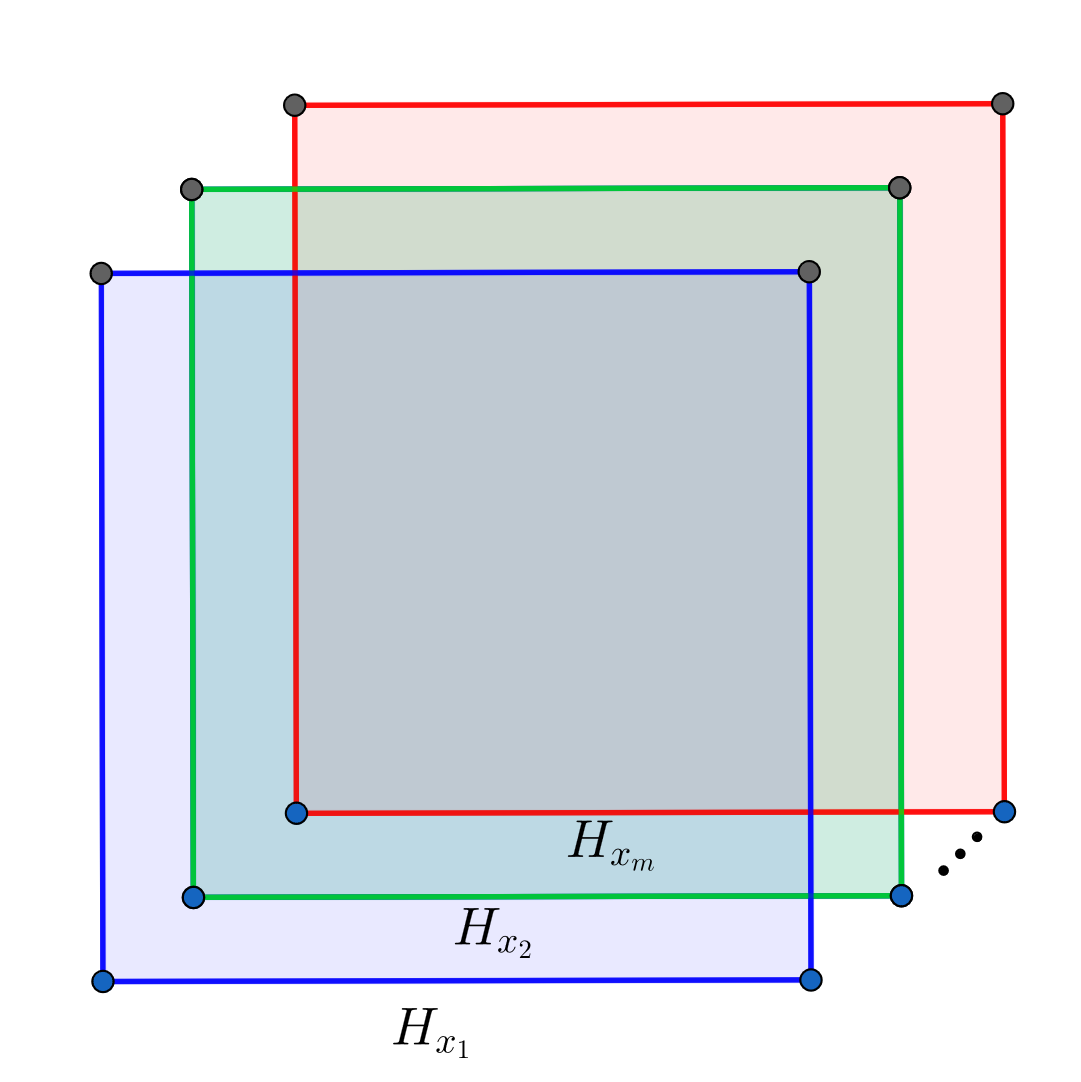
\includegraphics[width=0.4\textwidth, keepaspectratio]{../figs/Trajectory_Tensor_1}}
		 		\subfigure{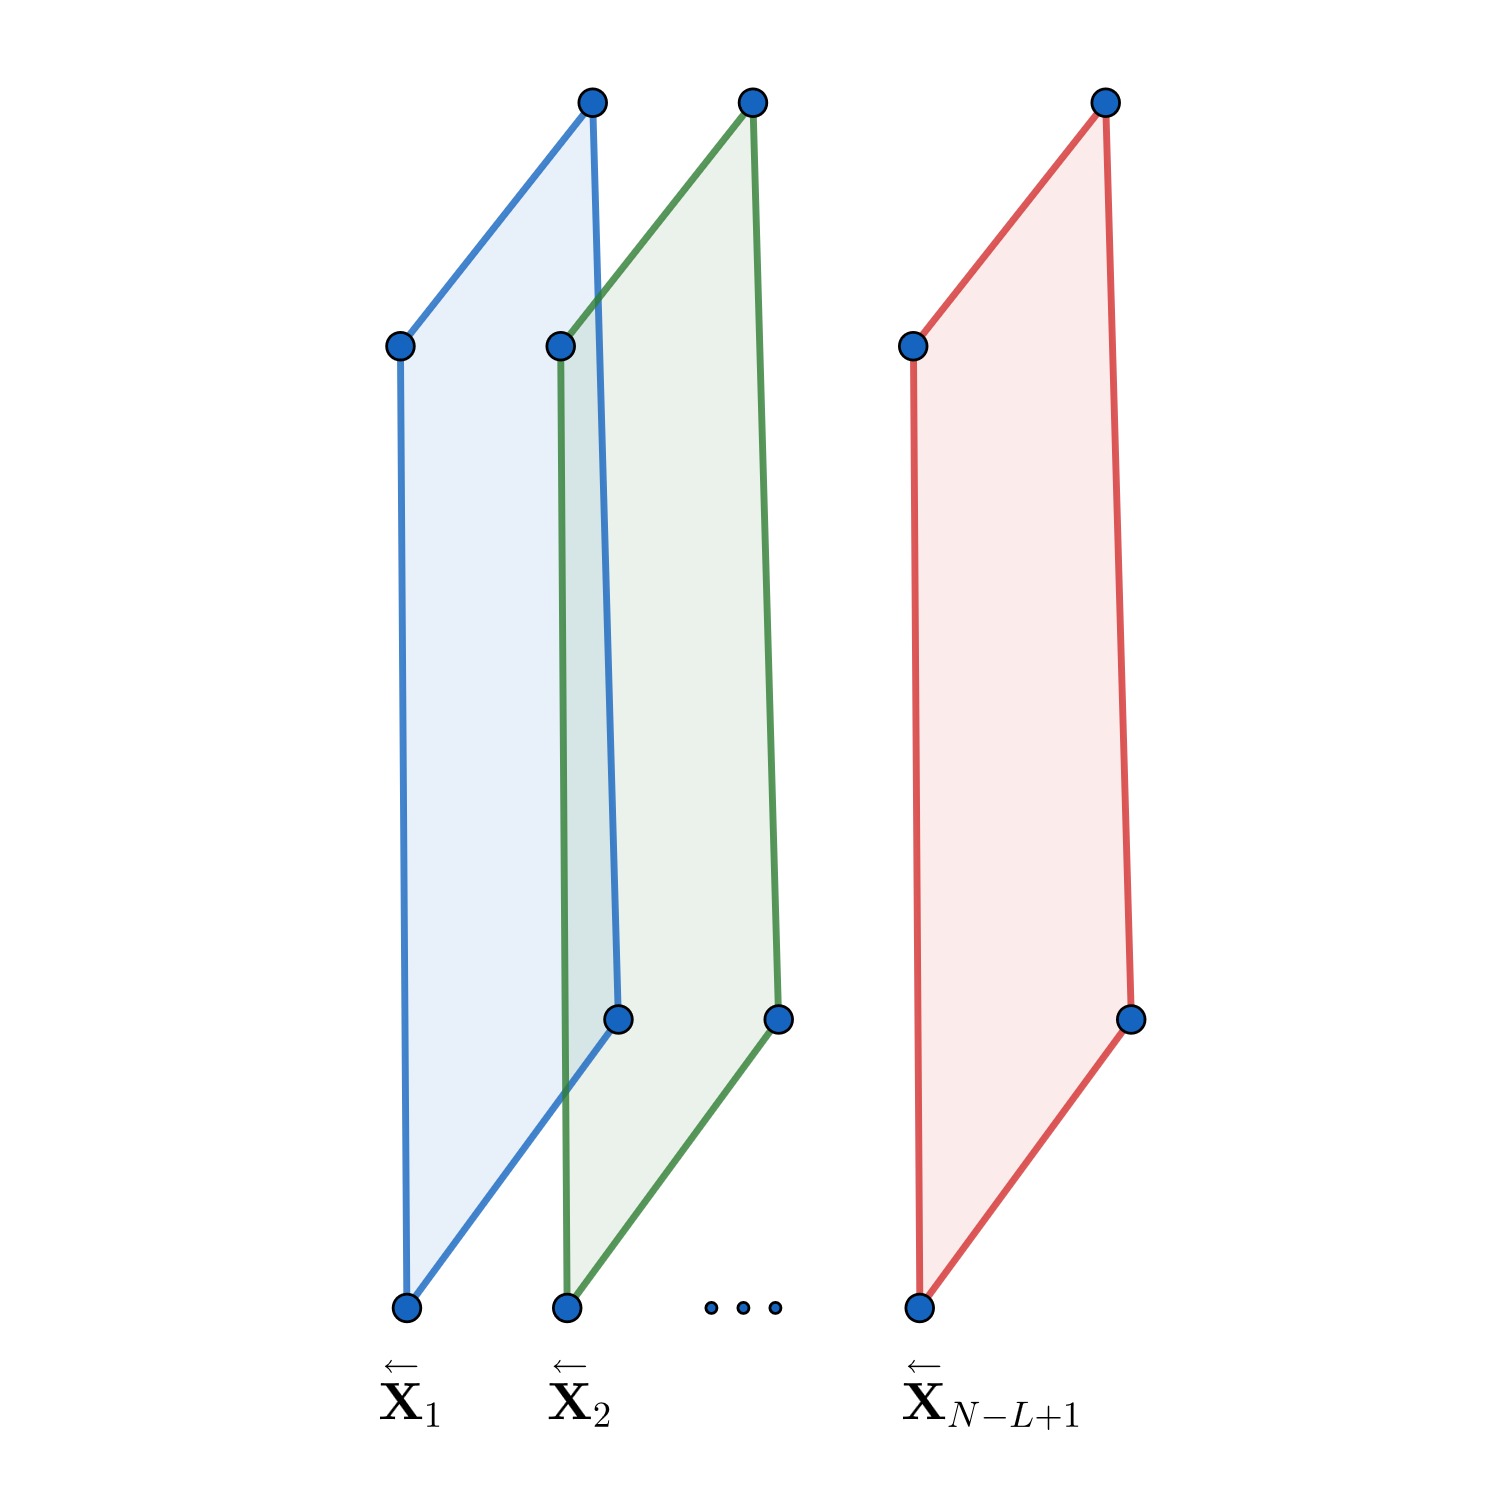
\includegraphics[width=0.4\textwidth, keepaspectratio]{../figs/Trajectory_Tensor_2}}
		 		
		 		\caption{Два вида на траекторный тензор. Слева --- в виде набора траекторных матриц сигналов $ \{x_i(t)\}_{i=1}^m $. Справа --- в виде набора матриц задержки.}\label{pic:traj_tensor}
		 	\end{figure}
	    
	    	В данном случае $ \boldsymbol{\phi}(\cdot) $ уже многомерное, а значит вместо вектора задержки одного сигнала необходимо рассматривать их набор для всех $ m $ сигналов в момент $ t $. Т.е. образами вложения будут служить \emph{матрицы задержки} $ ( \delayV{1_t} \ldots \delayV{m_t} ) := \delayM{t} $. Вместо же траекторной матрицы сигнала нужно рассматривать \textit{траекторный тензор} $ \mathbf{T} $ набора сигналов. Он складывается из матриц задержки, выстроенных подряд по второму измерению тензора, см. рис.\ref{pic:traj_tensor}. Из построения также следует, что $ \mathbf{T} $ является состыковкой траекторных матриц $ \mathbf{H}_{x_i} $ вдоль третьего измерения.
	    	
	    	Продолжая аналогию подраздела выше, мы получаем \emph{собственное пространство набора рядов} в виде линейной оболочки матриц задержек. Но нам интересно построить его для каждого сигнала отдельно.
	    	
	    	Выше мы обещали дать определение взаимосвязи рядов в рамках нашей модели. 
	    	
	    	\begin{Def}
	    		Мы называем набор временных рядов \emph{связанным}, если они имеют одинаковое для всех собственное пространство с единым базисом.
	    	\end{Def}
	    	
	    	Предъявим метод построения такого пространства и базиса. Заметим, что для этого достаточно разложить матрицы задержки каждого сигнала по общему набору векторов. Теперь применим \textit{CPD-разложение} к траекторному тензору и рассмотрим его вид для каждого сечения по третьему измерению:
	    	
	    	\begin{equation}\label{eq:tSSA_decomp}
	    		\mathbf{T} = \sum\limits_{i = 1}^{r} \mathbf{a}_i \otimes \mathbf{b}_i \otimes \mathbf{c}_i \Leftrightarrow \begin{cases}
	    			\mathbf{H}_{x_1} = \sum\limits^{r} \boldsymbol{\sigma}_{x_1}(i) \cdot \mathbf{a}_i  \mathbf{b}_i^{\mathsf{T}}  \\
	    			\mathbf{H}_{x_2} = \sum\limits^{r} \boldsymbol{\sigma}_{x_2}(i) \cdot \mathbf{a}_i  \mathbf{b}_i^{\mathsf{T}} \\
	    			\ldots \\
	    			\mathbf{H}_{x_m} = \sum\limits^{r} \boldsymbol{\sigma}_{x_m}(i) \cdot \mathbf{a}_i  \mathbf{b}_i^{\mathsf{T}} 
	    		\end{cases}
	    	\end{equation}
	    
	    	Проанализируем полученное. Разложение определяется каноническим тензорным рангом $ r $ и набором векторов, которые удобно упаковать в матрицы: $ A = [\mathbf{a}_1 \ldots \mathbf{a}_r]; B = [\mathbf{b}_1 \ldots \mathbf{b}_r]; C = [\mathbf{c}_1 \ldots \mathbf{c}_r] $, $ k $-ую строку матрицы $ C $ мы обозначаем $ \boldsymbol{\sigma}_{x_k} $. Она имеет смысл набора сингулярных чисел для $ \mathbf{H}_{x_k} $, только в данном случае они могут быть отрицательными. Из определения CPD как разложения вида (\ref{eq:tSSA_decomp}) c минимальным $ r $ следует, что матрицы $ A, B, C $ имеют полный ранг. Общим собственным пространством сигналов является $ \text{Lin}(\{\mathbf{a}_i\}) $ с единым базисом $ \{\mathbf{a}_i\}_{i = 1}^r $, в общем случае не ортогональным. В формулировке задачи мы предполагали, что размерность вложения не должна быть большой, т.е. $ r \ll L $. Наконец заметим, что строки матриц $ \mathbf{H}_{x_k} $ также являются векторами задержек размерности $ N - L + 1 $, и в их терминах общим пространством сигналов будет $ \text{Lin}(\{\mathbf{b}_i\}) $. Т.о. наш подход обладает согласованностью относительно выбора $ \delayV{k_t} $, чего, например, нет у метода mSSA.
	    	
	    	В данном разложении связь рядов определяют $ \boldsymbol{\sigma}_{x_k} $ : если для разных сигналов они имеют нулевые элементы в разных позициях, то собственные пространства будут различаться (т.к. в качестве базисных векторов будут участвовать разные наборы $ \mathbf{a}_i $).
	    	
	    \subsection*{Декомпозиция набора рядов}
	    
	    	Теперь мы можем представить каждый сигнал $ x_k(t) $ суммой компонент по следующему принципу: \emph{декомпозиция траекторной матрицы $ \mathbf{H}_{x_k} $ определяет декомпозицию временного ряда}. Эта методика лежит в основе метода SSA. Т.к. разложение у каждой матрицы своё, то и сигналы можно обрабатывать независимо.
	    	
	    	В данном подходе основным является свойство \emph{ганкелевости} траекторных матриц --- равенства элементов на одной антидиагонали. Каждому временному ряду длины $ N $ взаимнооднозначно сопоставляется ганкелева матрица $ L \times (N - L + 1) $.
	    	
	    	Для получения декомпозиции предполагается, что факторы разложения $ \mathbf{H}_{x_k} $ можно сгруппировать таким образом, что, сложив их в каждой группе, мы получим ганкелевы матрицы $ C_1, \ldots, C_s $. Это бы в точности соответствовало представлению $ x_k(t) $ в виде суммы $ s $ сигналов. На практике такая ситуация почти невозможна (см.~\cite{ecfb9dc578be43ae9ee8fc88b8ff9151}), поэтому все $ C_i $ дополнительно \emph{ганкелизируют} --- усредняют каждую антидиагональ. Будем обозначать эту операцию $ \text{Hankel}(\cdot) $. Описанная процедура представлена выражением (\ref{eq:decomp_method_ideal}).
	    	
	    	\begin{multline}\label{eq:decomp_method_ideal}
	    		\mathbf{H}_{x_k} = \sum\limits_{i = 1}^{r} \boldsymbol{\sigma}_{x_k}(i) \cdot \mathbf{a}_i  \mathbf{b}_i^{\mathsf{T}} = \sum\limits_{i \in \mathbb{I}_1} \boldsymbol{\sigma}_{x_k}(i) \cdot \mathbf{a}_i  \mathbf{b}_i^{\mathsf{T}} + \ldots + \sum\limits_{i \in \mathbb{I}_s} \boldsymbol{\sigma}_{x_k}(i) \cdot \mathbf{a}_i  \mathbf{b}_i^{\mathsf{T}} = \\ = C_1 + \ldots + C_s = \text{Hankel}(C_1) + \ldots + \text{Hankel}(C_s)  \Leftrightarrow x_k(t) = c_1(t) + \ldots c_s(t)
	    	\end{multline}
	    	
	    	Здесь $ \mathbb{I}_1 \sqcup \ldots \sqcup \mathbb{I}_s = \{1, \ldots, r\} $ --- выбранные группы индексов. Четвёрте равенство в (\ref{eq:decomp_method_ideal}) нуждается в обосновании, для этого докажем простое свойство оператора ганкелизации:
	    	
	    	\begin{Lem}
	    		Оператор $ \text{Hankel}(\cdot) $ линейный.
	    	\end{Lem}
	    	
	    	\begin{proof}
	    		Возьмём две матрицы $ A $ и $ B $ одного размера и рассмотрим их элементы с одной антидиагонали $ a_1, \ldots, a_n $ и $ b_1, \ldots, b_n $. Тогда соответствующая антидиагональ в $ \text{Hankel}(A + B) $ равна $ \dfrac{1}{n} \sum\limits^n (a_i + b_i) = \dfrac{1}{n} \sum\limits^n a_i + \dfrac{1}{n} \sum\limits^n b_i $, т.е. равна сумме антидиагоналей матриц $ \text{Hankel}(A) $ и $ \text{Hankel}(B) $.
	    	\end{proof}
	    	
	    	Учитывая, что $ \mathbf{H}_{x_k} $ --- ганкелева, мы полностью обосновали корректность процедуры построения декомпозиции временного ряда.
	    	
	    	Несмотря на это, хочется группировать факторы так, что каждая матрица $ C_i $ была как можно более "ганкелевой". Это соответствует изначальной идее о связи разложений матриц и сигналов, а также повышает интерпретируемость компонент.    Для дальнейшей оптимизации группировки введём меру "гакелевости".
	    	
	    	\begin{Def}
	    		\emph{Невязкой ганкелизации} матрицы $ \mathbf{H} $ назовём $ \text{r}(\mathbf{H}) = \lVert \mathbf{H} - \text{Hankel}(\mathbf{H}) \rVert_{F}^2 $ 
	    	\end{Def}
	    	
	    	В статистическом плане, эта невязка соответствует суммарной дисперсии антидиагоналей матрицы.
	    	
	    	Теперь для поиска декомпозиции ряда будем искать разбиение факторов, наилучшее в плане средней ганкелевой невязки:
	    	
	    	\begin{gather*}
	    		\frac{1}{s} \sum\limits_{j = 1}^s \text{r}(C_s) \to \min \\
	    		\begin{cases*}
	    			C_j = \sum\limits_{i \in \mathbb{I}_j} \boldsymbol{\sigma}_{x_k}(i) \cdot \mathbf{a}_i  \mathbf{b}_i^{\mathsf{T}}, \  \forall j = 1 \ldots s \\
	    			\mathbb{I}_1 \sqcup \ldots \sqcup \mathbb{I}_s = \{1, \ldots, r\} \\
	    			s \in \{2 \ldots r\}
	    		\end{cases*}
	    	\end{gather*}
	    	
	    	В итоге имеем задачу дискретной оптимизации по множеству всех разбиений и, скорей всего, для неё нет быстрого алгоритма поиска решения [TODO NP-hard]. Поэтому предлагается следующая эвристика: имея оптимальное разбиение на данное число групп, продолжать разбивать каждую из них на две оптимальным внутри этой группы способом. Так можно продолжать до получения достаточного числа компонент. Данный принцип проиллюстрирован на рис.\ref{pic:decomp_conception}. С точки зрения декомпозиции исходного ряда мы получаем его оптимальное разбиение на две компоненты, а затем продолжаем декомпозировать их независимо друг от друга. Получаем рекурсивную процедуру \emph{DichotomyPartition}, которую можно адаптивно перезапускать для получения нужного количества компонент:
	    	
	    	\begin{lstlisting}[language=Python, caption={Псевдокод процедуры рекурсивного получения декомпозиции временного ряда},]
	    		def DichotomyPartition(num_components):
	    			"""
	    			Args:
	    			num_components: how many components from initial signal
	    							 							is desired 
		    		
	    			Returns:
	    			factor groups related to best signal decomposition
	    			"""
	    			# at the start we have one group of factors,
	    			# which forms hankel trajectory matrix
	    			partition_list = [[1, 2, 3, ..., r]]
	    			mean_hankel_resid = 0
	    			
	    			# proceed until we obrain enough groups
	    			while len(partition_list) < num_components:
	    				new_partition_list = []
	    		
	    				# disect each group into two optimally within this group
	    				# FullSearch test all possible partitions into 2 groups
	    				# and find best in terms of Mean Hankel Residual
	    				for partition in partition_list:
	    					sub_partition_1, sub_partition_2 = FullSearch(partition)
	    		
	    					new_partition_list.extend(sub_partition_1, sub_partition_2)
	    		
	    				# calculate Mean Hankel Residual of new partition 
	    				mean_hankel_resid = CalculateResidual(new_partition_list)
	    				
	    				yield new_partition_list, mean_hankel_resid
	    				
	    				# save new partition
	    				partition_list = new_partition_list    		
	    	\end{lstlisting}
	    	
	    	\begin{figure}[h!]
	    		\centering
	    		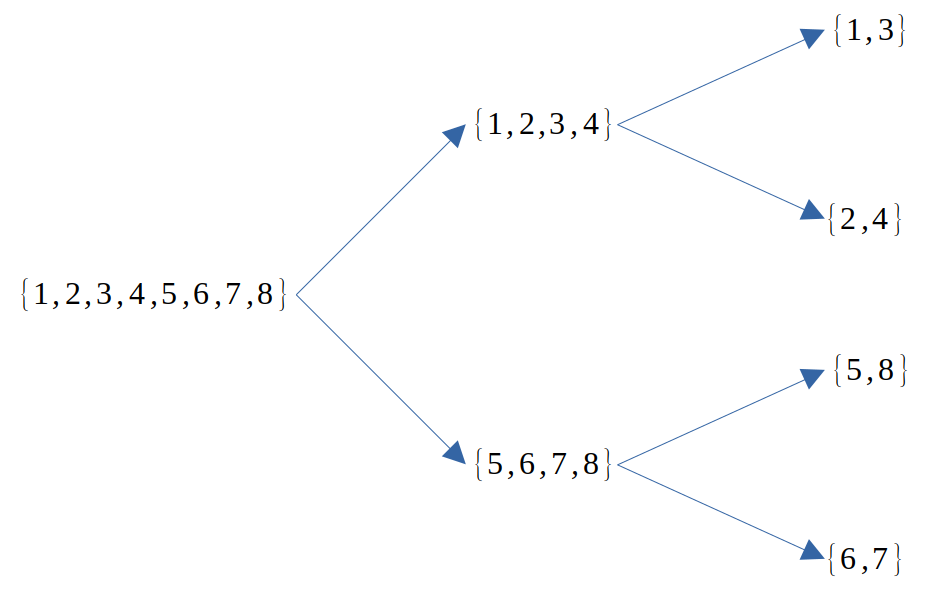
\includegraphics[width=0.6\textwidth, keepaspectratio]{../figs/dichotomy_drawings/factors.png}    
	    		
	    		$ \Updownarrow $
	    				
	    		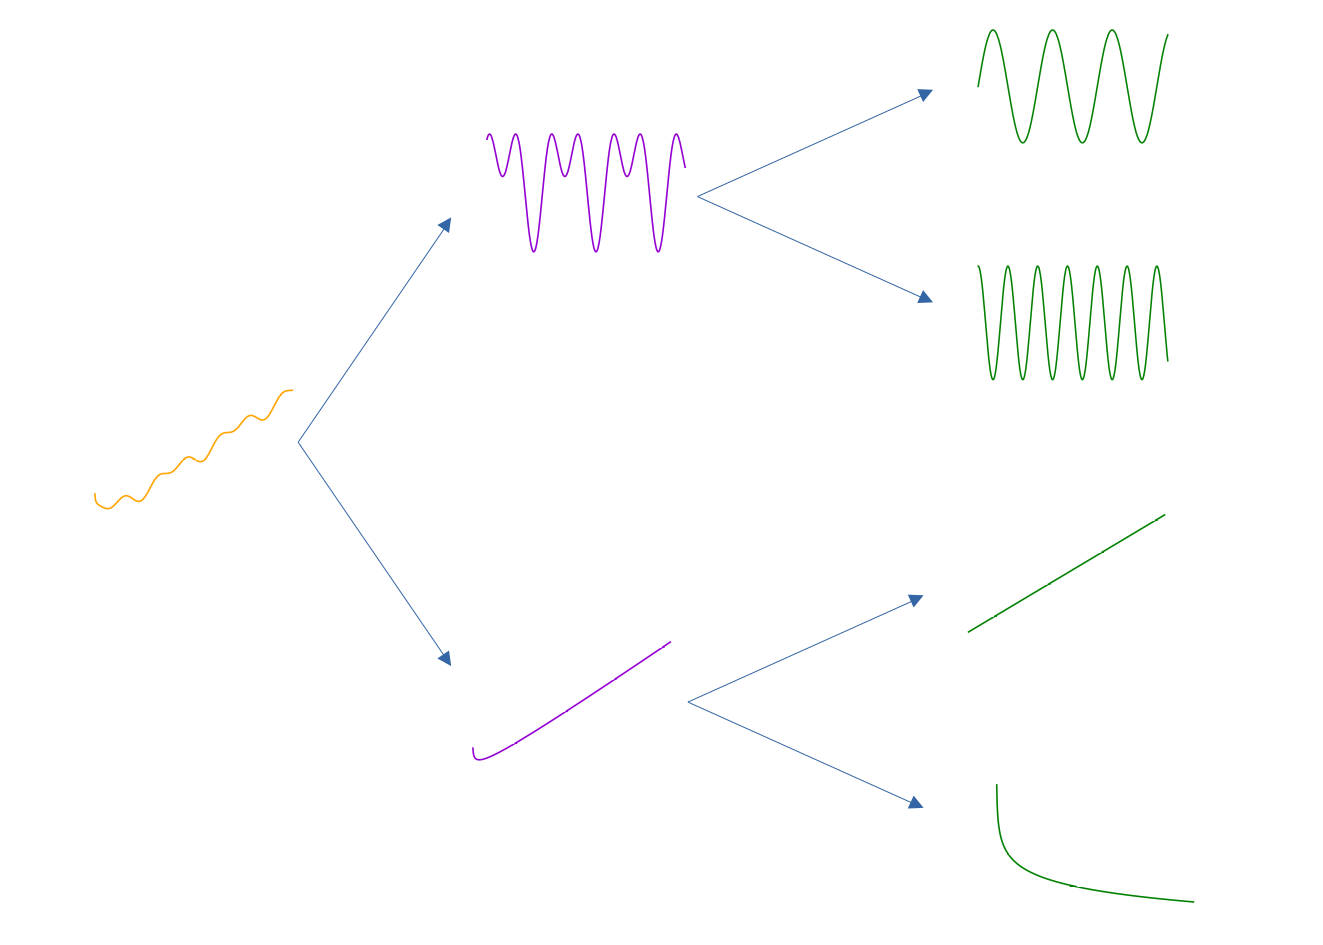
\includegraphics[width=0.6\textwidth, keepaspectratio]{../figs/dichotomy_drawings/signals.png}	
	    		
	    		\caption{Пример рекурсивного разбиения факторов (в виде индексов) на 4 группы. На каждом уровне ищется оптимальное разбиение внутри уже построенных группировок. С точки зрения разложения временных рядов мы рекурсивно раскладываем каждую полученную на данном уровне компоненту на две подкомпоненты.}\label{pic:decomp_conception}
	    	\end{figure}
	    	
	    \subsection*{Прогноз для набора рядов}
	     
	    	Получение прогноза в нашей модели сводится к восстановлению компонент векторов задержек каждого входного ряда. Т.к. мы построили общий для всех сигналов базис $ \{\mathbf{a}_i\}_{i = 1}^r $, то каждый сигнал может обрабатываться независимо.
	    	
	    	Если бы $ \{\mathbf{a}_i\}_{i = 1}^r $ был ортогональным, то мы бы могли применить технику прогнозирования SSA \cite{ecfb9dc578be43ae9ee8fc88b8ff9151}. Наша модель не даёт такой гарантии, поэтому метод SSA необходимо модифицировать.
	    	
	    	Рассмотрим произвольный входной ряд $ x(t) $ и построим для него прогноз на один шаг вперёд. Вектор задержки $ \delayV{N + 1} = (x(N - L) \ldots x(N + 1))^{\mathsf{T}} $, в котором последняя компонента неизвестна, лежит в пространстве $ \text{Lin}(\{\mathbf{a}_i\}) $. В терминах вводимой ранее матрицы $ A \in \mathbb{R}^{L \times r} $ полного ранга это записывается:
	    	
	    	\begin{gather}\label{eq:main_pred_for_A}
	    		\delayV{N + 1} = A \boldsymbol{\lambda} \Leftrightarrow \begin{cases}
	    			\mathbf{x}_{kn} = A_{kn} \boldsymbol{\lambda}  \\
	    			x(N + 1) = \mathbf{a}_{pr}^{\mathsf{T}} \boldsymbol{\lambda}
	    		\end{cases}, \text{ где } \\
	    		A = \left( \dfrac{A_{kn}}{\mathbf{a}_{pr}^{\mathsf{T}}} \right) \nonumber \\
	    		\delayV{N + 1} = (\mathbf{x}_{kn} \  x(N + 1))^{\mathsf{T}} \nonumber
	    	\end{gather}
	    	
	    	Здесь $ \boldsymbol{\lambda} \in \mathbb{R}^r $, вектор задержки и матрица представлены в блочном виде для отделения известной части сигнала и его будущего значения. Т.о. для прогноза необходимо найти $ \boldsymbol{\lambda} $ из первой части системы (\ref{eq:main_pred_for_A}). Матрица данной СЛАУ $ A_{kn} \in \mathbb{R}^{(L - 1) \times r} $ имеет ранг не менее $ r - 1 $, но даже пусть ранг будет полный. Сама система в силу предположения модели $ r \ll L $ является переопределённой. Значит, решение здраво искать только в смысле метода наименьших квадратов: $ \boldsymbol{\lambda} = (A_{kn}^T A_{kn})^{-1} A_{kn}^T \mathbf{x}_{kn} $. В итоге прогноз модели даётся формулой:
	    	
	    	\begin{equation}\label{eq:tssa_pred}
	    		x(N + 1) = \mathbf{a}_{pr}^{\mathsf{T}} (A_{kn}^T A_{kn})^{-1} A_{kn}^T \mathbf{x}_{kn}
	    	\end{equation}
	    
	    	 Здесь $ \mathbf{a}_{pr}^{\mathsf{T}} (A_{kn}^T A_{kn})^{-1} A_{kn}^T = \mathbf{d}^{\mathsf{T}} $ --- вектор-строка, и, вычислив её один раз, можно быстро строить предсказания на несколько шагов, последовательно получая $ x(N + 1), x(N + 2), $  и т.д.
	    	 
	    	 Если расписать (\ref{eq:tssa_pred}) в терминах $ x(t) $:
	    	 
	    	 \begin{equation*}\label{eq:autoregr}
	    	 	x(t) = \sum\limits_{i = 1}^{L - 1} d_i \cdot x(t - i)
	    	 \end{equation*}
	    	 
	    	 Получаем, что предсказание методом tSSA, по-сути, сводится к \textit{авторегрессионной} модели ряда $ AR(L - 1) $. Соответственно, поведение прогноза полностью определяется коэффициентами $ d_i $.
	    
	\section{Эксперимент}	
			
		
		\newpage
		\printbibliography
	
\end{document}